\documentclass[10pt, conference, compsocconf]{IEEEtran}

\usepackage{color}
\usepackage{soul}

%\documentclass[a4paper, UKenglish]{lipics}
%\usepackage{amsmath}
%\theoremstyle{plain}

\usepackage{subfigure}
\usepackage{hyperref}
\usepackage{graphicx}
\usepackage{amssymb}
\usepackage{amsmath}
\usepackage{times}
\let\proof\relax % undefine the environment
\let\endproof\relax
\usepackage{amsthm}

\usepackage{xspace}
\usepackage{algorithm}% http://ctan.org/pkg/algorithm
\usepackage[noend]{algpseudocode}% http://ctan.org/pkg/algorithmicx

\newcommand{\todo}[1]{\color{red}\textbf{\hl{\{ #1 \}}}\color{black}\xspace}
\newcommand{\ceil}[1]{\left\lceil #1 \right\rceil}
\newcommand{\floor}[1]{\left\lfloor #1 \right\rfloor}

\begin{document}
\title{Space-Time Kernel Density Estimation}


\maketitle

\section{Introduction}

The rapid propagation of infectious diseases (e.g. zika, Ebola, H1N1,
dengue fever) is conducive to serious, epidemic outbreaks, posing a
threat to vulnerable populations. Such diseases have complex
transmission cycles, and effective public health responses require the
ability to monitor outbreaks in a timely
manner~\cite{eisen2011using}. Space-time statistics facilitate the
discovery of disease dynamics including rate of spread, seasonal
cyclic patterns, direction, intensity (i.e. clusters), and risk of
diffusion to new regions.  However, obtaining accurate results from
space-time statistics is computationally very demanding, which is
problematic when public health interventions are promptly needed. The
issues of computational efforts are exacerbated with spatiotemporal
datasets of increasing size, diversity and
availability~\cite{grubesic2014spatial}. High-performance computing
reduces the effort required to identify these patterns, however
heterogeneity in the data must be accounted for~\cite{Hohl16}. 


Epidemiology is only one of the application domains where it is
important to understand how events occurring at different locations and
different times form clusters. Political analysis, social media
analysis, or the study of animal migration also require the
understanding of spatial and temporal locality of events. The massive
amount of data we see nowadays is often analyzed using complex
models. But before these can be constructed, data scientists  need to
interactively visualize and explore the data to understand its
structure. 


\section{Space-Time Kernel Density Estimation}
\label{sec:stkde}

\subsection{Description}

Space-time kernel density (STKDE) is used for identifying
spatiotemporal patterns in datasets. It is a temporal
extension of the traditional 2D kernel density
estimation~\cite{Silverman86} which generates density surface
(``heatmap'') from a set of $n$ points located in a geographic space. The resulting density
estimates are visualized within the space-time cube framework using two spatial $(x,
y)$ and a temporal dimension $(t)$~\cite{Nakaya10}. STKDE creates a discretized 3D
 volume where each voxel (3D equivalent of a pixel) is assigned a
density estimate based on the surrounding points. The space-time
density is estimated using (following the notations
of~\cite{Hohl16}):

$$ \hat{f} (x, y, t) = \frac{1}{n h_s^2 h_t} \sum_{i | d_i < h_s, t_i<h_t}
k_s (\frac{x-x_i}{h_s},\frac{y-y_i}{h_s}) k_t(\frac{t-t_i}{h_t})$$

Density $\hat{f} (x, y, t)$ of each voxel is determined by number and distance of events (points)
$(x_i, y_i, t_i)$ within its vicinity, which is conceptualized by a
cylinder. The spatial bandwidth $h_s$ forms a circle which, due to the
orthogonal relationship between space and time, is extended to a
cylinder by temporal bandwidth $h_t$. For every event inside the
cylinder, the spatial ($d_i$) and temporal ($t_i$) distances are smaller
than $h_s$ and $h_t$. Therefore, the event receives a weight based on the
kernel functions $k_s$ and $k_t$ (distance decay):

$$k_s (u,v) = \frac{\pi}{2} (1-u)^2 (1-v)^2$$
$$k_t (w) = \frac{3}{4} (1-w)^2$$

Figure~\ref{fig:stkde-ex} illustrates how varying the bandwidths used
in STKDE helps focusing the graphical visualization of Dengue fever
cases in Cali, Colombia~\cite{Delmelle14}. Figure~\ref{fig:stkde} shows the impact
of a single point on the neighboring space.

\begin{figure}
  \subfigure[$h_s = 2500m$, $h_t = 14 days$]{\includegraphics[width=.49\linewidth]{Dengue-2500-14.pdf}}
\subfigure[$h_s=500m$, $h_t = 7 days$]{\includegraphics[width=.49\linewidth]{Dengue-500-7.pdf}}
  \caption{Visualization of Dengue fever cases in Cali, Colombia in
    2010 and 2011 for different spatial bandwidth and temporal bandwidth.}
  \label{fig:stkde-ex}
\end{figure}

\begin{figure}
  \centering
  \includegraphics[width=.5\linewidth]{stkde.pdf}
  \caption{The computation of STKDE happens in a domain space of size
    $g_x,g_y,g_t$. Each point impacts the neighboring space at a
    distance $h_s$ in space and $h_t$ in time; forming a cylinder of
    diameter $2 h_s$ and of height $2 h_t$.}
  \label{fig:stkde}
\end{figure}

Computationally, the domain of size $g_x$, $g_y$, $g_t$ is discretized
in voxels using a spatial resolution $sres$ and a temporal resolution
$tres$. Therefore, the domain is represented by a grid of size
$G_x=\ceil{\frac{g_x}{sres}}$, $G_y=\ceil{\frac{g_y}{sres}}$,
$G_t=\ceil{\frac{g_t}{tres}}$. Each point causes a density increase in
the voxels that are within a cylinder centered on the point, of
radius equal to the spatial bandwidth in voxels
$H_s=\ceil{\frac{h_s}{sres}}$, and of half height equal to the
temporal bandwidth $H_t=\ceil{\frac{h_t}{tres}}$.

All the notations are summarized in Table~\ref{tab:notation}. As a
convention all uppercase notations denote quantities in voxels and all
lowercase notations denote quantities in domain space.

\begin{table}
  \centering
  \begin{tabular}{|l|l|}
    \hline 
    $n$ & Number of points\\
    $s = (x,y,t)$ & A voxel and sampling coordinate\\
    $(x_i, y_i, t_i)$ & Coordinate of point $i$\\
    $h_s$, $h_t$ & Spatial and temporal bandwidth \\ 
    $g_x, g_y, g_t$ & Real size of the domain (in meters) \\
    \hline
    $sres$, $tres$ & Resolution (in meters) \\
    $s = (X,Y,T)$ & A voxel in voxel space\\
    $(X_i, Y_i, T_i)$ & Voxel of point $i$\\
    $G_x, G_y, G_t$ & Size of the domain (in voxels)\\
    $H_s, H_t$ & Bandwidth (in voxels) \\
    \hline 
  \end{tabular}
  ~
  \caption{Notations}
  \label{tab:notation}
\end{table}



\subsection{Gold Standard Implementation}

The gold standard implementation follows the exact definition of STKDE
as it is given above. It is a voxel-based algorithm we call VB. For
each voxel, VB finds the points within the temporal and spatial bandwidths and calculates the contribution
to the density of this voxel. The pseudo code is given in Algorithm~\ref{alg:vb}.

\begin{algorithm}
\caption{\textsc{VB}}
\scriptsize
\begin{algorithmic}
\For{all voxels $s=(x,y,t)$}
\State $sum = 0$
  \For{all points $i$ at $x_i, y_i, t_i$}
    \If{$\sqrt{(x_i-x)^2+(y_i-y)^2}< h_s$ and $|t_i-t| \leq h_t$}
    \State $sum += k_s(\frac{x-x_i}{h_s},\frac{y-y_i}{h_s}) k_t(\frac{t-t_i}{h_t})$
    \EndIf
  \EndFor
  \State $stkde[X][Y][T] = \frac{sum}{n h_s^2h_t}$
\EndFor
\end{algorithmic}
\label{alg:vb}
\end{algorithm}


The algorithm performs $\theta(G_x G_y G_t n)$ distance tests and
computes $\theta(n H_s^2 H_t )$ densities. Since $H_s$ is smaller than
$G_x$ and $G_y$ and since $H_t$ is smaller than $G_t$, the complexity of the
algorithm is $\theta(G_x G_y G_t n )$ and it requires $\theta(G_x G_y G_t)$
memory.


\bibliographystyle{alpha}
\bibliography{ipdps}

\end{document}


